\section{Zweite Iteration}\label{sec:pro2}

In \autoref{sec:pro1} haben sich während der Testphase des ersten Prototyps sowohl neue Probleme als auch fehlende Funktionalitäten identifizieren lassen.
Diese sollen bei der Entwicklungs eines zweiten Prototyps in diesem Abschnitt berücksichtigt werden. \\

\subsection{Observation}
Um einen Überblick über die Test-Ergebnisse aus dem vorherigen Abschnitt herzustellen und eventuelle Ursachen zu identifizieren, werden diese im Nachfolgenden zunächst aufgelistet und anschließend weiter ausgewertet:

\begin{enumerate}
  \item Systemzustand nicht intuitiv erkennbar (\emph{Floating Action Buttons})
  \item Text- und Formelemente auf Tablets nicht gut lesbar bzw. benutzbar
  \item Eingetragenen Messwerte auf dunekelem Hintergrund nicht gut erkennbar
  \item Zuordnen von Gerüsttypen zu Formen nicht möglich
  \item Zuschneiden und Rotieren des Bildes nicht möglich
\end{enumerate}

\noindent
Zunächst aufgefallen ist, dass beide Testpersonen in \autoref{subsec:test1} die \emph{Floating Actions Buttons} als Hindernis bei der Benutzung der App beschrieben haben.
Dadurch, dass die \emph{Buttons} zu jeder Zeit immer nur ein Icon anzeigen, und erst beim Klick auf diese erkennbar wird, welche weiteren Aktionen möglich sind, wird dem Nutzer nur wenig bis keine Rückmeldung über den aktuellen Systemzustand und ausführbare Aktionen gegeben.
Dies ist ein Verstoß gegen Nielsen-Heuristik \autoref{itm:N1} und spiegelt sich direkt in einer negativen Nutzungserfahrung der App wieder. \\

Ein weiterer Punkt, der in \autoref{subsec:test1} negativ aufgefallen ist, ist die Benutzung auf einem Tablet-Gerät.
So ist die Nutzung der App auf Endgeräten mit einer höheren Pixeldichte mühsam, und eine Quelle für Fehler.
Da Text- und Formelemente, die auf kleineren Bildschirm ohne Probleme zu erkennen und bedienen sind, auf größeren Bildschirmen nicht skaliert werden, sind diese bei einer höheren Pixeldichte nur mühsam erkennbar, und sorgen so für eine negative Benutzererfahrung und bieten gleichzeitig eine Quelle für potentielle Fehler. \\ 
\todo{Nielsen reffen}

Die schlechte Lesbarkeit von eingetragenen Messwerten bei Bildern mit einem dunkelen Hintergrund hängt vermutlich damit zusammen, dass die Textfarbe unabhängig von den Bildeigenschaften auf Grau festgelegt ist.
So führt die graue Textfarbe in Kombination mit einem fehlenden Texthintergrund, besonderns bei Bildern dunkelerem Hintergrung, zur schlechten Lesbarkeit der Messwerte. \\
\todo{Nielsen reffen}

Beim Testen der App ergab sich für beide Testpersonen außerdem das Problem, dass diese nach Funktionen gesucht haben, die nicht in der App vorhanden sind.
\todo{Wie fehlende Funktionen hier beschreiben?}
nach einer Funktion gesucht wurde, um eingetragene Formen mit bereits vorhandenen Gerüsttypen zu verknüpfen, oder Bilder beim Import in die gewünschte Größe und Form zu bringen.
Das Fehlen dieser Funktionen hat sich negativ auf das Benutzungserlebnis ausgewirkt, da die Benutzer fest davon ausgegangen sind, dass diese in der App integriert seien.

\subsection{Idea Generation}\label{subsec:idea2}
\todo{refs auf papers/guidelines wie bei Konzeption}
Um dem Benutzer jederzeit eine klare und einfache Rückmeldung über den aktuellen Systemzustand und die darin ausführbaren Aktionen zu geben, bietet es sich an, eine Art Statusleiste am unteren Bildschirmrand zu verankern.
Diese soll mit Hilfe von unterscheidbaren, aber intuitiv verständlichen Icons, über den aktuellen Modus (Zeichnen oder Text) informieren, und zugleich nicht benutzbare Aktionen nicht auswählbar gestalten. \\

Für eine bessere und einfachere Benutzung der App auf Tablet-Geräten bietet es sich einerseits an, eine zweite Benutzeroberfläche, die nur bei Geräten mit einer Displaybreite von beispielsweise mindestens $600$ Pixeln benutzt wird, einzubinden. 
Andererseits besteht die Möglichkeit, die Größe diverser Text- und Formelemente mit der Bildschirmgröße zu skalieren.
Dies hat den Effekt, dass Bildschirm-Elemente bei verschiedenen Bildschirmgrößen ungefähr gleich groß sind. \\

Die schlechte Erkennbarkeit von eingetragenen Messwerten auf Bildern mit dunkelem Hintergrund lässt sich durch die Benutzung eines Texthintergrundes lösen.
So könnte, wie bei \emph{Toasts}, die im Android System seit API X vorhanden sind, ein dunkeler Hintergrund in Kombination mit einer hellen Textfarbe dazu genutzt werden, eingetragene Messwerte unabhängig von den Lichtverhältnissen im Bild gut erkennbar zu machen. \\
\todo{ref auf toast}

Um Formen direkt den passenden Gerüsttypen zuzuordnen, bietet sich ein modaler Dialog an, der zum Beispiel bei einem langen Klick auf die gewünschte Form angezeigt wird, und in einem \emph{Dropdown} vorhandene Gerüsttypen zur Auswahl anzeigt.
Falls ein langer Klick auf die Form zu unintuitiv ist, würde sich eine Option in der oben beschriebenen Statusleiste anbieten, die nur dann auswählbar ist, wenn eine Form markiert ist. \\

Das Schneiden und Rotieren von Bildern kann einerseits durch die Benutzung der in der Android API vorhandenen \emph{Crop-Activity} realisiert werden, andererseits würde sich auch die Benutzung einer dedizierten \emph{Android-Library} für das Schneiden von Bildern anbieten.
Ersteres bringt die Gefahr mit sich, dass die Verfügbarkeit einer solchen \emph{Crop-Activity} im Android-System vom Gerätehersteller und der verwendeten Android-Version abhängig ist, sodass die Funktion nicht auf allen Geräten funktioieren wird. \todo{ref auf API docs}

\subsection{Prototyping}

Der zweite Prototyp wurde am 3. Januar 2018 fertiggestellt, und umfasst die Implementierung der in \autoref{subsec:idea2} gesammelten Ideen. \\

So wurde die Statusleiste durch eine \emph{Bottom-Bar} am unteren Bildschirmrand umgesetzt (siehe \autoref{fig:bar2}).

\begin{figure}[ht]
  \begin{subfigure}[t]{0.4\textwidth}
    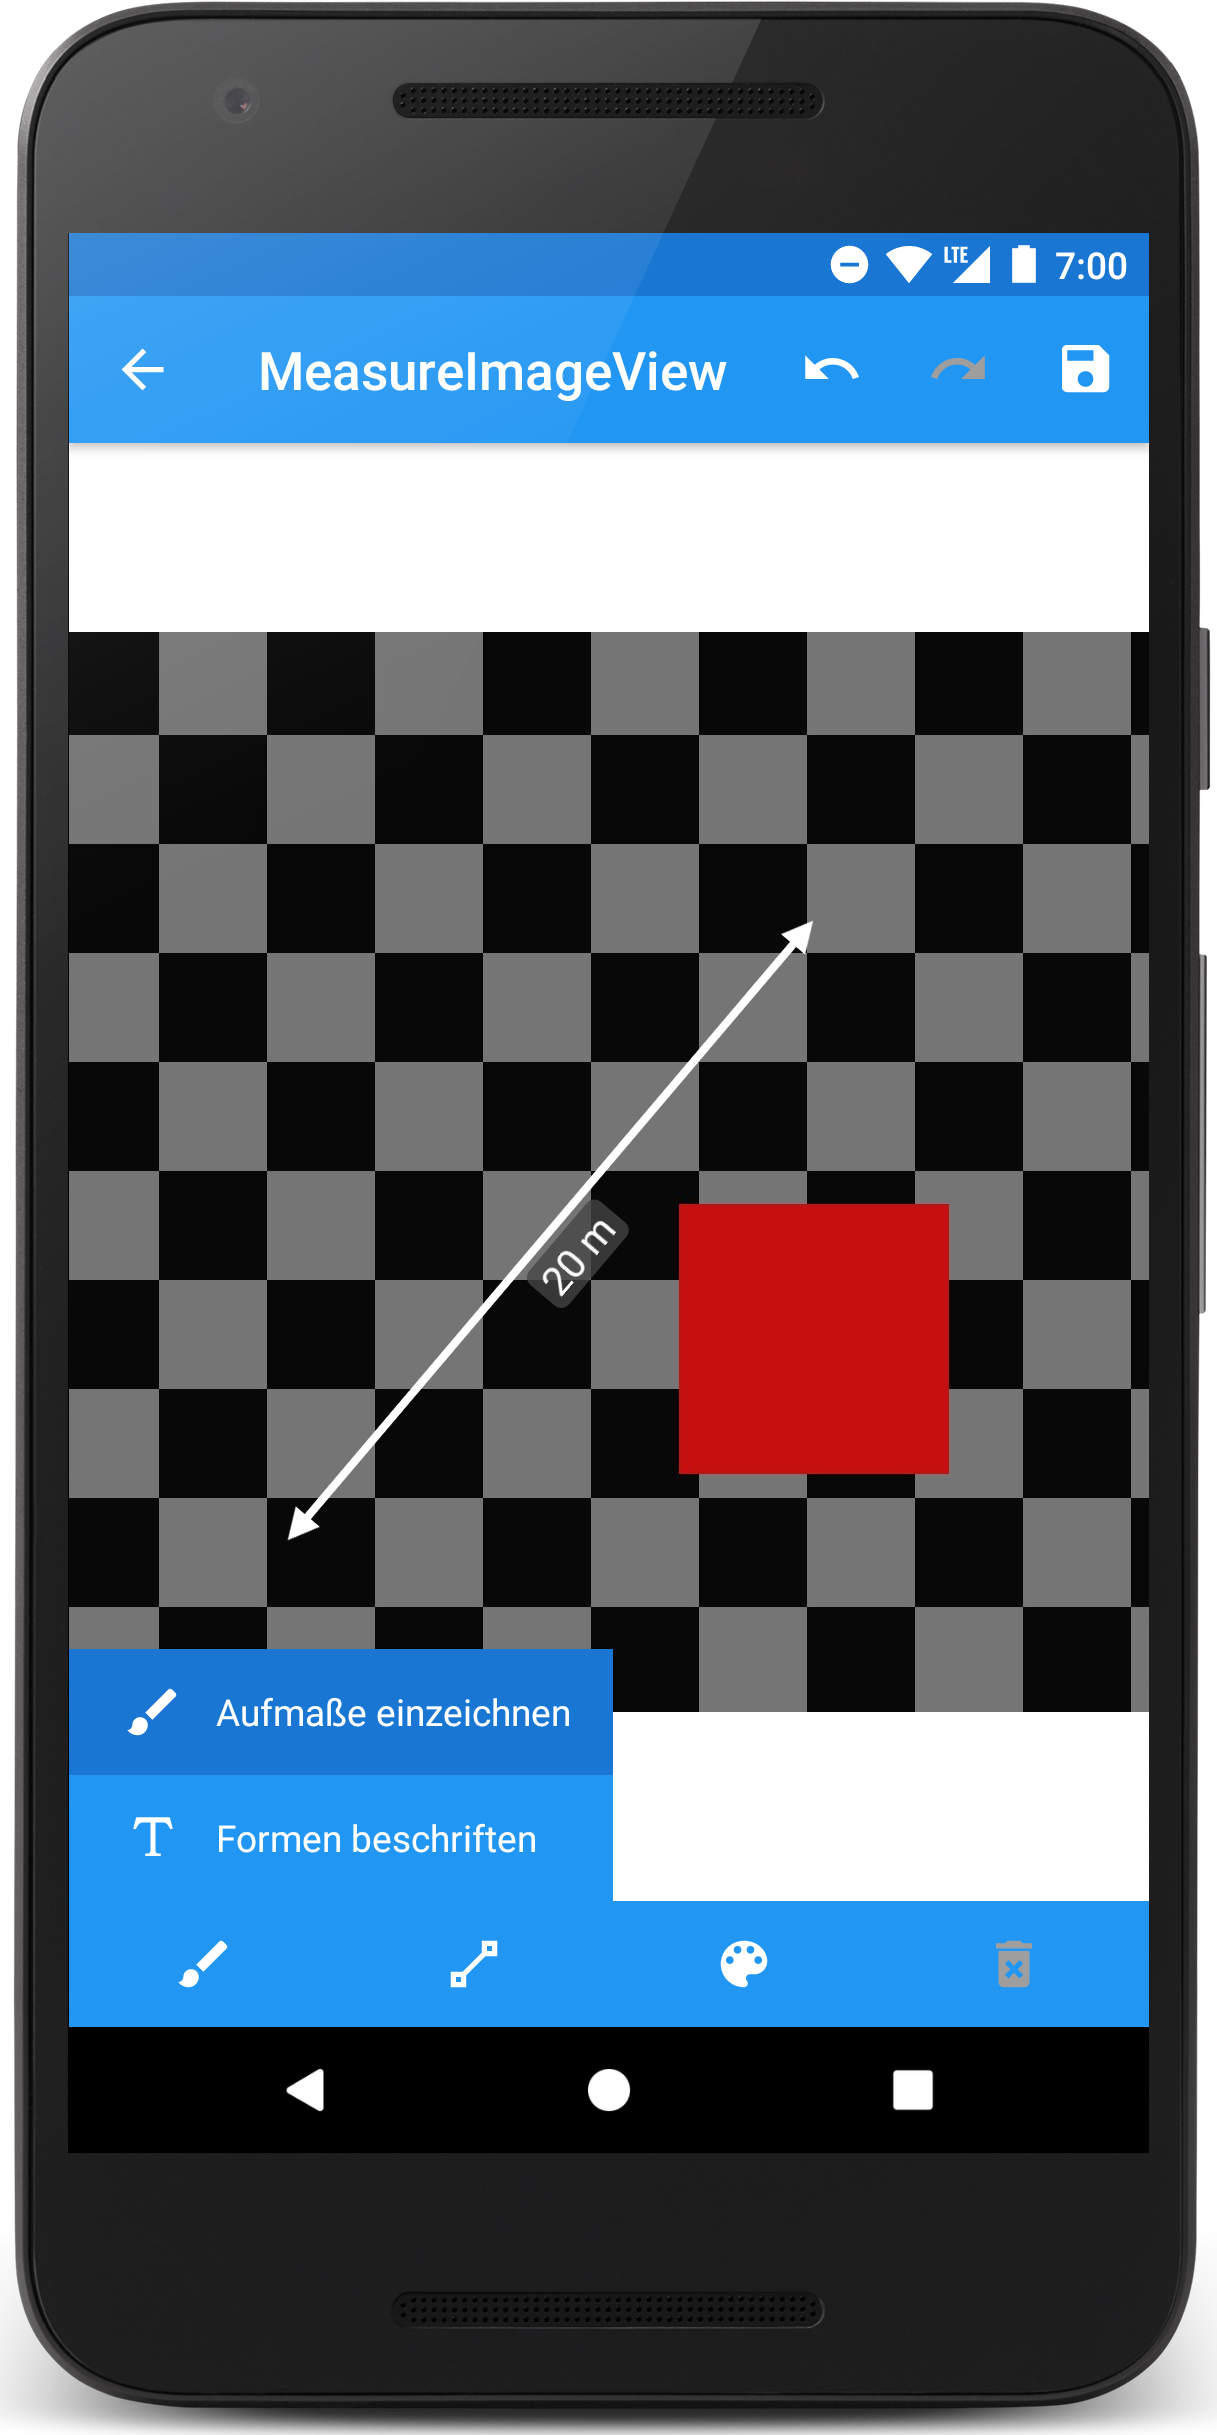
\includegraphics[keepaspectratio, width=\textwidth]{prototype2/expanded_mode}
    \caption{Statusleiste im Zeichen-Modus mit Popup-Dialog zur Auswahl des Modus}
    \label{fig:mode2}
  \end{subfigure}
  \begin{subfigure}[t]{0.4\textwidth}
    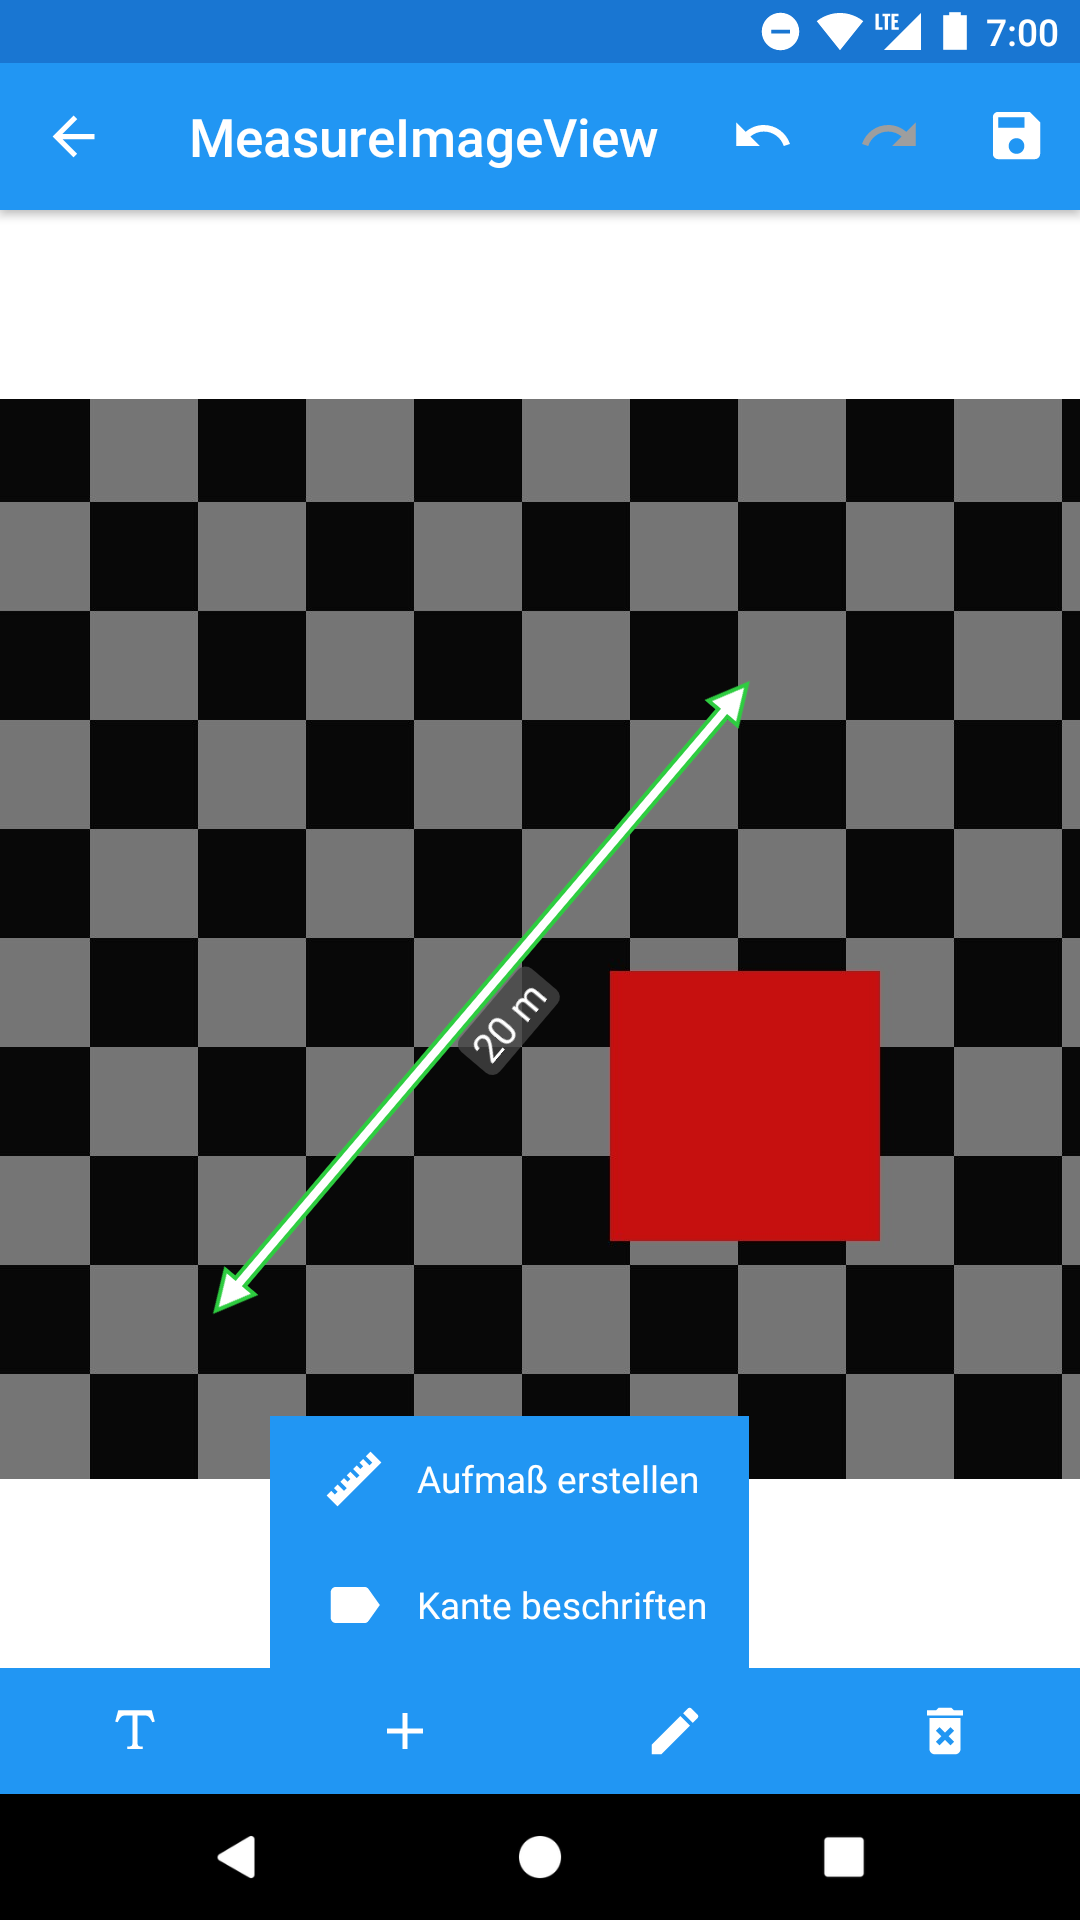
\includegraphics[keepaspectratio, width=\textwidth]{prototype2/label_popup}
    \caption{Statusleiste im Text-Modus mit Popup-Dialog zur Beschriftung der ausgewählten Form}
    \label{fig:labelp2}
  \end{subfigure}
  \centering
  \caption{Bedienung der Statusleiste im zweiten Prototyp}
  \label{fig:bar2}
\end{figure}

\noindent
Diese besteht aus vier verschiedenen Icons, die nur dann auswählbar sind, wenn die entsprechende Aktion im aktuellen Systemzustand durchgeführt werden kann.
Das Icon ganz links ermöglicht das Wechseln zwischen dem Zeichen- und Textmodus (siehe \autoref{fig:mode2}). \\

Im Zeichenmodus kann per Klick auf das zweite Icon über ein \emph{Popup-Menü} die gewünschte Form ausgewählt werden. 
Im selben Modus kann beim Klick auf das dritte Icons (Farbpalette) die gewünschte Formfarbe im Voraus konfiguriert werden. Hierzu öffnet sich, wie schon beim ersten Prototyp, ein modaler Farbauswahl-Dialog.
In beiden Modi ermöglicht das vierte Icon (Mülleimer) das Löschen von ausgewählten Formen bzw. Texten. \\

Im Textmodus kann beim Klick auf das zweite Icon über ein \emph{Popup-Menü} entweder eine ausgewählte Form mit einer Kantenbeschriftung versehen, oder mit einem Gerüsttyp verknüpft werden (siehe \autoref{fig:labelp2}).
Das dritte Icon ermöglicht das Bearbeiten von bereits eingetragenen Messwerten und verknüpften Gerüsttypen.
Auch in diesem Modus sind die Icons nur dann auswählbar, wenn der aktuelle Systemzustand dies zulässt.
So sind das dritte und vierte Icons beispielsweise nur dann benutzbar, wenn zuvor eine Form ausgewählt worden ist. \\

Für eine einfache und fehlerfreie Benutzung auf Tablet-Geräten wurden sämtliche Größen mit Hilfe von dichteunabhängigen Pixeln modelliert, wie sie in den \emph{Android-Developer Guides} vorgeschlagen werden \citep{DP18}.
So werden hierbei alle Maße in der Einheit \emph{dp} angegeben, welche zur Laufzeit vom System in normale Pixel (\emph{px}) umgewandelt werden.
Die genaue Umformung lautet dabei wie folgt:
$$
px =  dp \times (\frac{dpi}{160})
$$

wobei $dp$ für ``dots per inch'' steht.
Dies stellt sicher, dass auf Geräten mit einer hohen Pixeldichte Elemente nicht zu klein dargestellt werden. \\
\todo{Bild vorher nachher Resize Points}

Messwerte sind mit einem grau-gefärbten Rechteck hinterlegt, welches dafür sorgt, dass sich die Texte besser vom Hintergrund abheben, und so auch bei schwierigen Bedingungen klar lesbar sind.  \\
\todo{Bild vorher nachher}

Das Zuordnen von Gerüsttypen zu gezeichneten Formen wurde mit Hilfe eines modalen Dialogs umgesetzt, der neben dem Gerüsttyp auch noch Textfelder für die verschiedenen Dimensionen des Gerüsts besitzt.
Hierdurch kann der Benutzer nicht nur den Gerüsttyp, sondern auch Maße des Gerüsts, welche im Bild aufgrund des Aufnahmewinkels eventuell nicht zu sehen sind, eintragen und in den Meta-Daten speichern. \\
\todo{Bild von Dialog}

Für das Schneiden und Rotieren von Bildern vor dem Annotieren wurde \emph{uCrop}, eine dedizierte Android-Library, welche auf \emph{Github} als Open-Source Projekt unter der \emph{Apache License Version 2.0} vorhanden ist, in das Projekt eingebunden \citep{UC18}.
Diese bietet im Gegensatz zu der \emph{Crop-Activity}, welche von manchen Android-Versionen zur Verfügung gestellt wird, Unterstützung für alle Gerätehersteller ab der Android-Version $14$ an.
Außerdem erlaubt diese Library das Anpassen sämtlicher Farben der Benutzeroberfläche, sodass Konsistenz beim Einbinden in den Prototyp bestehen bleibt, und der Nutzer nicht von zwei völlig verschiedenen Farbpaletten überrascht wird. \todo{Bilder}

\subsection{Testing}\label{subsec:test2}
Der zweite Prototyp wurde sechs Tage lang, bis zum 9. Januar 2018, von den beiden Geschäftsführern in ihrem Arbeitsalltag getestet.
Das anschließende Feedback ergibt sich aus einem Gespräch am 9. Januar. \\

Als deutlich positive Verbesserung wurde dabei von beiden Testpersonen die neue Statusleiste am unteren Bildschirmrand genannt.
Hierdurch sei die Benutzung der App um einiges leichter gefallen, als beim ersten Prototyp mit den \emph{Floating Action Buttons}. \\

Jedoch sei, so die beiden Tester, das initiale Einarbeiten in die App immer noch zu schwierig, und nicht intuitiv genug.
Hier fehlte beiden Testpersonen eine Hilfestellung, die beim Start der App die wichtigsten Funktionen zusammenfasst, und kurz erklärt wozu was benutzt werden kann. \\

Ein weiteres Problem, dass beim Testen des Prototyps aufgefallen sei, ist der Farbdialog.
Dieser sei nach Aussage einer Testperson, zu fortgeschritten und biete eine Auswahl an Farben, die ``[...] der normale Gerüstbauer niemals verwendet wird'' \todo{Zitat hier?}
Dies ist ein Problem, welches während der Test-Phase zum ersten Prototyp nicht als solches identifiziert wurde, sich jetzt aber doch als Problem herausgestellt hat.
Hierbei wäre es laut Testpersonen nämlich sinnvoller, den Benutzer ``[...] nicht mit so vielen Auswahlmöglichkeiten zu überfordern [...]'', sondern eine übersichtliche Menge an häufig benutzten Farben direkt auswählbar zu machen. \\

Außerdem wurde sich neben einem einfacheren Farbdialog eine Funktion gewünscht, Freitexte ins Bild einzutragen zu können. 
Dies sei laut der Aussage beider Testpersonen ein wichtiger Aspekt, da beim bisherigen Erstellen der Aufmaße oftmals weitere Notizen oder Kommentare auf Skizzen eingetragen werden, um besondere Punkte bzw. Abmachungen festzuhalten. \\

Zudem fehle die Möglichkeit, Linien mit nur einer Pfeilspitze zu zeichnen.
Dies sei laut beider Testpersonen wichtig, um Längen, die auf dem Bild nur einen Startpunkt haben, und in die Tiefe offen sind, zu kennzeichnen. \\

Des Weiteren seien verlinkte Gerüsttypen an Formen nicht intuitiv durch den Indikator, wie er in dem ersten Prototyp umgesetzt wurde, erkennbar.
Zusätzlich wurde angemerkt, dass die Textfelder im Dialog zum Verlinken des Gerüsttyps durchaus sinnvoll seien, aber nur selten genutzt wurden, da sich Messwerte gemerkt werden müssen, um diese anschließend in den Dialog einzutragen. \\
